%%%%%%%%%%%%%%%%%%%%%%%%%%%%%%%%%%%%%%%%%%%%%%%%%%%%%%%%%%%%%%%%%%%%%%%%%%%%%%%%
%                                                                              %
%   PAW   - Reference Manual -- LaTeX Source                                   %
%                                                                              %
%   Chapter 2: General principles                                              %
%                                                                              %
%   EPS file      : pawtut02.eps                                               %
%                   pawppoverview1.eps                                         %
%                   pawppoverview2.eps                                         %
%                   pawtut10.eps                                               %
%                                                                              %
%   Editor: Michel Goossens / IT-ASD                                           %
%   Last Mod.: 30 July 1998 Olivier Couet                                      %
%                                                                              %
%%%%%%%%%%%%%%%%%%%%%%%%%%%%%%%%%%%%%%%%%%%%%%%%%%%%%%%%%%%%%%%%%%%%%%%%%%%%%%%%

\chapter{General principles}
\label{sec:PRINCIP}
\newcommand{\RZ}{{\sf RZ}\index{RZ}}
\newcommand{\PHIGS}{{\sf PHIGS}\index{PHIGS}}
\newcommand{\GPHIGS}{{\sf GPHIGS}\index{GPHIGS}}
\newcommand{\XPAW}{{\sf PAW}\index{PAW (Physics Analysis Workstation)}}
\newcommand{\PS}{{\sf Post\-Script}\index{PostScript}}
\newcommand{\EPS}{{\sf En\-cap\-su\-la\-ted Post\-Script}\index{PostScript!Encapsulated}}
\newcommand{\FALCO}{{\sf FALCO}\index{FALCO}}
\newcommand{\MSDOS}{{\sf MSDOS}\index{MSDOS}}
\newcommand{\MAC}{{\sf MacIntosh}\index{MacIntosh}}
\newcommand{\GDDM}{{\sf GDDM}\index{GDDM}}
\newcommand{\XW}{{\sf X Window System}\index{X Window System}}
\newcommand{\Xxi}{{\sf X11}\index{X11}}
\newcommand{\GL}{{\sf GL}\index{GL}}
\newcommand{\GPR}{{\sf GPR}\index{GPR}}
\newcommand{\GMR}{{\sf GMR}\index{GMR}}
\newcommand{\MOTIF}{{\sf Motif}\index{Motif}}
\newcommand{\XLIB}{{\sf Xlib}\index{Xlib}}

\newcommand{\NDC}{normalized device coordinates\index{coordinates!normalized device}}
\newcommand{\DC}{device coordinates\index{coordinates!device}}
\newcommand{\WC}{world coordinates\index{coordinates!world}}

\newcommand{\ndc}{{\sf NDC}\index{coordinates!normalized device}}
\newcommand{\dc}{{\sf DC}\index{coordinates!device}}
\newcommand{\wc}{{\sf WC}\index{coordinates!world}}

\newcommand{\FORTRAN}{{\sf Fortran}\index{Fortran}}
\newcommand{\CHARACTER}{{\tt CHARACTER}}

\newcommand{\UGP}{underlying graphics package\index{underlying graphics package}}
\newcommand{\UGPs}{underlying graphics packages\index{underlying graphics package}}

\newcommand{\HW}{{\tt higz\_windows.dat}\index{higzwindows.dat}}

\newcommand{\nt}{{\sf NT}\index{normalization transformation}}
\newcommand{\wt}{{\sf WT}\index{workstation transformation}}

\newcommand{\NT}{normalization transformation\index{normalization transformation}}
\newcommand{\NTs}{normalization transformations\index{normalization transformation}}
\newcommand{\WT}{workstation transformation\index{workstation transformation}}
\newcommand{\WTs}{workstation transformations\index{workstation transformation}}
\newcommand{\ASCII}{{\tt ASCII}\index{ASCII}}

\newcommand{\UNIX}{{\sf UNIX}\index{UNIX}}
\newcommand{\VMS}{{\sf VAX/VMS}\index{VAX/VMS}}

\newcommand{\MB}{{\bf Main Browser}\index{Main Browser}}
\newcommand{\EW}{{\bf Executive Window}\index{Executive Window}}
\newcommand{\TP}{{\bf Transcript Pad}\index{Transcript Pad}}
\newcommand{\IP}{{\bf Input Pad}\index{Input Pad}}
\newcommand{\NV}{{\bf Ntuple Viewer}\index{Ntuple Viewer}}
\newcommand{\HSP}{{\bf Histogram Style Panel}\index{Histogram Style Panel}}
\newcommand{\PL}{{\bf PAW++ Locate}\index{PAW++ Locate}}
\newcommand{\GW}{{\bf Graphics Window}\index{Graphics Window}}
\newcommand{\CE}{{\bf Cut Editor}\index{Cut Editor}}

\section{Access to PAW}
\label{sec:PACCESS}\index{PAW!access}
 
At CERN the PAW program
is interfaced on all systems via a command
procedure which gives access to the three release levels of
the CERN Program Library
(\texttt{PRO}duction, \texttt{OLD} and the \texttt{NEW} areas) and
sets the proper environment if necessary.
Users who are not at CERN or who are using non-central
computer systems should contact their system
administrator for help on PAW.
\index{CERN Program Library!OLD}
\index{CERN Program Library!NEW}
\index{CERN Program Library!PRO}

\subsection{VAX/VMS}
\index{VAX}
\index{VMS}
 
A command file \texttt{CERN_ROOT:\lsb EXE\rsb PAW.COM}
is defined system-wide via the logical
symbol \texttt{PAW}; its interface is:

\begin{alltt}
      \Ucom{PAW/ver}\rmfamily\qquad(the default is \texttt{PRO})
\end{alltt}

You may set the initialization of PAW either as a \texttt{PAWLOGON.KUMAC}
located in your home directory, or through the
logical symbol \texttt{DEFINE PAW\$LOGON disk:\lsb user.subdir\rsb file.kumac}
to be defined usually in your \texttt{LOGIN.COM}.

\subsection{Unix systems}
\index{Apollo}
\index{unix}
 
The driver shell script is located in the file
\texttt{/cern/pro/bin/paw}.
In order to access it automatically you could add the
directory \texttt{/cern/pro/bin} to your command search path.
\index{path}%
\index{command!search path}%
\index{HELP}%
\index{X windows}%
\index{X11}%
\index{display}%
\index{host}%
\index{workstation}%
\index{Domain}%
\index{version}%
\index{PAWLOGON}%
The command syntax is:
\begin{alltt}
      \Ucom{paw -v ver}\rmfamily\qquad(the default is \texttt{-v PRO})
\end{alltt}

\subsection{Workstation type}
 
PAW needs to know the X-host where graphics must be
displayed; this can be specified on each system on the command line:
\begin{alltt}
      Vax/VMS:   \Ucom{PAW/X11/host=yourhost}
      Unix:      \Ucom{paw -d X11 -h yourhost}
\end{alltt}
or at the ``\texttt{Workstation}'' prompt in PAW:
\texttt{Workstation type (?=HELP) \lsb CR\rsb =1 : \Ucom{1.yourhost}}
 
If \texttt{yourhost} is not specified, the output is redirected (like for all
X11 applications) to the display defined via the environment variable 
{\tt DISPLAY}.

The workstation type selects which type of workstation has to be opened. 
It corresponds to a line number in a file \texttt{higz_windows.dat}.
PAW tries to open this file in your current working directory.
If it does not succeed it tries in your HOME directory.
If it doesn't succeed once more, it creates the file in your HOME directory 
as follows:
\begin{verbatim}
                      0000 0000 0600 0600
                              .
                              .
                              .
                      0000 0000 0600 0600
\end{verbatim}
where the lines define each of the workstation types (from 1 to 10) with
the x-margin (left), y-margin (top), x-size (width) and y-size (height) of the
corresponding window in pixels.

For a more complete and up to date description you can refer to the PAW FAQs 
avaialable from the PAW web home page.

\subsection{Different modes to start PAW}

\begin{UL}
\index{batch}
\item A {\bf batch} version of PAW is available 
      (note that batch implies workstation type \texttt{0}):
\begin{alltt}
 On Unix   do:  \Ucom{paw -b macroname}
 On VMS    do:  \Ucom{PAW/BATCH=macroname}
\end{alltt}
\index{PAWLOGON}
\item One can {\bf disable} the automatic execution 
      of the \texttt{PAWLOGON} macro:
\begin{alltt}
 On Unix   do:  \Ucom{paw -n}
 On VMS    do:  \Ucom{PAW/NOLOG}
\end{alltt}
\end{UL}

\section{Initialising PAW}
\label{sec:INITIAL}
\index{PAW!initialisation}
 
When PAW is started, a {\bf system} startup
procedure is initiated, which indicates the current
version of PAW and requests the {\bf workstation type} of
the terminal or workstation which you are using.
\index{initialisation}
\index{workstation!type}
\begin{alltt}
\$ \Ucom{PAW}
 ******************************************************
 *                                                    *
 *            W E L C O M E    to   P A W             *
 *                                                    *
 *        Version 2.10/01       2 September 1998      *
 *                                                    *
 ******************************************************
 Workstation type (?=HELP) <CR>=1 : ?

 List of valid workstation types:
       0:  Alphanumeric terminal
    1-10:  Describe in file higz_windows.dat
  n.host:  Open the display on host (1 < n < 10)
    7878:  FALCO terminal
    7879:  xterm
\end{alltt}
Note that if you specify {\Ucom{0}},
PAW will not open a graphics workstation.
This may be appropriate if one wants to use PAW on an alphanumeric
terminal.
 
Before passing control to the user, the system looks for a user-supplied file
\texttt{pawlogon.kumac}.
The latter can contain
commands which the user wants to be executed at PAW startup, e.g.
declaration of files, creation of aliases, definition of HPLOT parameters.
\index{PAWLOGON}
A simple version of this PAW initialisation file, displaying date
and time, can be:

\begin{alltt}
mess '******************************************************'
mess '*                                                    *'
mess '*   Starting PAW session on '//$date//' at '//$time//'     *'
mess '*                                                    *'
mess '******************************************************'
\end{alltt}
 
In order to
only have one version of this file on VAX/VMS the user should define
a {\bf logical name} \texttt{PAW\$LOGON} in his
\texttt{LOGIN.COM},
as explained on the previous page.
The file \texttt{pawlogon.kumac} is taken in the current directory.

\section{Command structure}
\label{sec:COMSTRU}
\index{command!structure}
 
PAW is based on the KUIP\cite{bib-KUIP} User Interface package,
which can provide different types of dialogue styles:

\begin{UL}
\item Command mode,
      where the user enters a command line via the terminal keyboard.
\item Alphanumeric menu mode,
      where the command is selected from a list.
\item Graphics menu modes:\\
\index{menu}
\hspace*{1em}$\bullet$ 
Pull-down menus, fixed layout reflecting the command structure;\\
\index{pull-down menu}
\hspace*{1em}$\bullet$ 
Panels of function keys, interactive user definable multiple layouts.
\index{panel!menu}
\end{UL}

It is possible to change interactively from one style to another.
 
The general format of a PAW command line is:
\begin{alltt}
      \Ucom{command parameters}
\end{alltt}
The first part of the {\bf command} has the format:
\begin{alltt}
      \Ucom{object/verb}
\end{alltt}
where the {\bf object} is the item on which the action is performed
(e.g. \texttt{HISTOGRAM, VECTOR, NTUPLE})
and the \texttt{verb} is the action to be performed (e.g.
\texttt{CREATE, DELETE, PLOT}). 
In some cases the object needs to be
specified further (e.g. \Ucom{GRAPHICS/PRIMITIVE}),
while in other cases the verb's action needs to be clarified further
(e.g. \Ucom{CREATE/1D}).
\index{abbreviation}
\index{command!abbreviation}
All components can be {\bf abbreviated} to their shortest unambiguous form. 
For example the two following
lines will have the same effect of creating a vector \texttt{A} with
nine components:
\begin{alltt}
     \Ucom{VECTOR/CREATE A(9)}
{\rm or}
     \Ucom{VE/CR A(9)}
\end{alltt}
\index{command!parameter!mandatory}
\index{command!parameter!optional}
In the case that the form is ambiguous all possible interpretations
for the given abbreviation are displayed.
 
The second part of a command are its {\bf parameters} and their meaning
is determined by their {\bf position}.
\index{mandatory parameter}
\index{optional parameter}
Some of these can be {\bf mandatory}
with the remaining ones {\bf optional}.
If all mandatory parameters are not provided on the command line,
PAW will prompt the user to specify them, indicating
the default values if defined.
If the user wants
to assign the default value to a parameter from the command line
he can use the {\bf place-holder} character
{\bf exclamation mark (!)} to signify this to PAW.
\index{place-holder!exclamation mark character}
\index{exclamation mark character!place-holder}
In the case of optional parameters, the user {\bf must} provide them
in the correct sequence if he wants to {\bf change} their values,
otherwise the corresponding defaults are taken.
Parameters containing blanks must be enclosed within single quotes.
 
In the example below we create a one-dimensional histogram,
providing the parameters one by one answering the PAW query:
\begin{alltt}
      PAW > \Ucom{histogram/create/1dhisto}
      Histogram Identifier (<CR>= ): \Ucom{10}
      Histogram title (<CR>= ): \Ucom{title1}
      Number of channels (<CR>=100): \Ucom{<CR>}
      Low edge (<CR>=0): \Ucom{10.}
      Upper edge (<CR>=100): \Ucom{20.}
\end{alltt}
For the command below
we provide all parameters on the command line, including
an optional one (\texttt{1000.}),
which by default has the value \texttt{0}.
Note that this parameter {\bf must} be specified
explicitly, since PAW {\bf does not} prompt for it,
as seen in the previous example.
Note also the use of the exclamation mark to take the default for the
number of channels (\texttt{100}).
\begin{alltt}
      PAW > \Ucom{hi/cr/1d 20 title2 ! 10. 20. 1000.}
\end{alltt}

\section{Getting help}
\label{sec:GETHELP}
 
Once inside PAW, one can start entering commands.
An interesting first try would be the \Ucom{HELP} command,
\index{HELP}
which displays a list of items, preceded by a number
and followed by one line of explanation.
In the next example we search for a command to
create a one-dimensional histogram.
\begin{falltt}
      PAW > \Ucom{help}
 
From  /...

 1:   KUIP          Command Processor commands.
 2:   MACRO         Macro Processor commands.
 3:   VECTOR        Vector Processor commands.
 4:   HISTOGRAM     Manipulation of histograms, Ntuples.
 5:   FUNCTION      Operations with Functions. Creation and plotting.
 6:   NTUPLE        Ntuple creation and related operations.
 7:   GRAPHICS      Interface to the graphics packages HPLOT and HIGZ.
 8:   PICTURE       Creation and manipulation of HIGZ pictures.
 9:   ZEBRA         Interfaces to the ZEBRA RZ, FZ and DZ packages.
10:   FORTRAN       Interface to MINUIT, COMIS, SIGMA and FORTRAN
                    Input/Output.
11:   NETWORK       To access files on remote computers.
12:   OBSOLETE      Obsolete commands.

Enter a number ('Q'=command mode): \Ucom{4} 

   /HISTOGRAM

   Manipulation of histograms, Ntuples.  Interface to the HBOOK package.


From  /HISTOGRAM/...

 1: * FILE          Open an HBOOK direct access file.
 2: * LIST          List histograms and Ntuples in the current directory.
 3: * DELETE        Delete histogram/Ntuple ID in Current Directory
                    (memory).
 4: * PLOT          Plot a single histogram or a 2-Dim projection.
 5: * ZOOM          Plot a single histogram between channels ICMIN and
                    ICMAX.
 6: * MANY_PLOTS    Plot one or several histograms into the same plot.
 7: * PROJECT       Fill all booked projections of a 2-Dim histogram.
 8: * COPY          Copy a histogram (not Ntuple) onto another one.
 9: * FIT           Fit a user defined (and parameter dependent) function
                    to a histogram ID (1-Dim or 2-Dim) in the specified
                    range.
10:   2D_PLOT       Plotting of 2-Dim histograms in various formats.
11:   CREATE        Creation ("booking") of HBOOK objects in memory.
12:   HIO           Input/Output operations of histograms.
13:   OPERATIONS    Histogram operations and comparisons.
14:   GET_VECT      Fill a vector from values stored in HBOOK objects.
15:   PUT_VECT      Replace histogram contents with values in a vector.
16:   SET           Set histogram attributes.

Enter a number ('\'=one level back, 'Q'=command mode): \Ucom{11} 

   /HISTOGRAM/CREATE

   Creation ("booking") of HBOOK objects in memory.


From  /HISTOGRAM/CREATE/...

 1: * 1DHISTO       Create a one dimensional histogram.
 2: * PROFILE       Create a profile histogram.
 3: * BINS          Create a histogram with variable size bins.
 4: * 2DHISTO       Create a two dimensional histogram.
 5: * PROX          Create the projection onto the x axis.
 6: * PROY          Create the projection onto the y axis.
 7: * SLIX          Create projections onto the x axis, in y-slices.
 8: * SLIY          Create projections onto the y axis, in x-slices.
 9: * BANX          Create a projection onto the x axis, in a band of y.
10: * BANY          Create a projection onto the y axis, in a band of x.
11: * TITLE_GLOBAL  Set the global title.

Enter a number ('\'=one level back, 'Q'=command mode): \Ucom{1}
 
 * /HISTOGRAM/CREATE/1DHISTO  ID TITLE NCX XMIN XMAX \lsb  VALMAX \rsb
 
   ID         C 'Histogram Identifier' Loop
   TITLE      C 'Histogram title' D=' '
   NCX        I 'Number of channels' D=100
   XMIN       R 'Low edge' D=0.
   XMAX       R 'Upper edge' D=100.
   VALMAX     R 'Maximum bin content' D=0.

   Create a one dimensional histogram.  The contents are set to zero.  If
   VALMAX=0, then a full word is allocated per channel, else VALMAX is used
   as the maximum bin content allowing several channels to be stored into
   the same machine word.

<CR>=continue, 'Q'=command mode, 'X'=execute: \Ucom{q}
\end{falltt}
An item preceded by a {\bf star} indicates
a {\bf terminal leaf} in the command tree,
i.e. an {\bf executable} command.
 
One can also inquire about {\bf creating a one-dimensional histogram}
by typing simply:
\begin{alltt}
      \Ucom{HELP histogram/create/1dhisto}
{\rm or}
      \Ucom{HELP his/cre/1d}
{\rm or even}
      \Ucom{HELP 1}
\end{alltt}
The system will then display the following information:
\begin{falltt}
  * /HISTOGRAM/CREATE/1DHISTO  ID TITLE NCX XMIN XMAX \lsb  VALMAX \rsb
 
   ID         C 'Histogram Identifier' Loop
   TITLE      C 'Histogram title' D=' '
   NCX        I 'Number of channels' D=100
   XMIN       R 'Low edge' D=0.
   XMAX       R 'Upper edge' D=100.
   VALMAX     R 'Maximum bin content' D=0.

   Create a one dimensional histogram.  The contents are set to zero.  If
   VALMAX=0, then a full word is allocated per channel, else VALMAX is used
   as the maximum bin content allowing several channels to be stored into
   the same machine word.
\end{falltt}

\subsection{Usage}
 
Very often a single line description of the usage of a command 
is sufficient as a reminder. 
This can be obtained by the \Ucom{USAGE} command, e.g.:
\index{USAGE command}
\begin{alltt}
      PAW > \Ucom{USAGE 1d}
 
      * /HISTOGRAM/CREATE/1DHISTO  ID TITLE NCX XMIN XMAX \lsb  VALMAX \rsb
\end{alltt}

\section{Special symbols for PAW}
\label{sec:SPESYMB}
 
\index{symbols}
\index{special symbols}
One should pay attention to the fact that, 
in addition to their common arithmetic meaning,
the symbols in table \ref{tab:KUIPSYS} 
have a special connotation when working with PAW .

\begin{table}[!h]
\begin{center}
\begin{tabular}{|>{\tt}l|l|}
\hline
\multicolumn{1}{|c|}{\bf Symbol} &
\multicolumn{1}{c|}{\bf Meaning}                                        \\
\hline
blank & Separator between command and parameter and between different
        parameters                                                      \\
/     & Separator between command elements                              \\
*     & Comment line (if first character of the command line)           \\
|     & Inline comments                                                 \\
'     & String delimiter                                                \\
\us   & Line continuation in KUIP commands                              \\
\commat& Escape character to be put in front of \texttt{|} and \texttt{'}
         to interpret them as literal                                   \\
!     &  Place-holder for command parameter (i.e. default value is taken)\\
      &  At beginning of command line: Unix C shell-like {\bf history}  \\ 
      &  (e.g. \texttt{!!, !number, !-number, !string})                    \\
\lsqb  \rsqb & Macro argument delimiters                                \\
\num  & Separator between macro file and macro member                   \\
( )   & Vector subscript delimiters                                     \\
:     & Vector subscript range                                          \\
,     & Multi-dimensional vector subscript dimensions delimiter         \\
\hline
\multicolumn{2}{|l|}{{\bf Note:} These special characters
loose their effect when imbedded in single quotes.}                     \\
\hline
\end{tabular}
\end{center}
\caption{Special symbols}
\label{tab:KUIPSYS}
\end{table}

\section{PAW entities and their related commands}
\label{sec:ENTITY}

\begin{figure}[!h]
\centering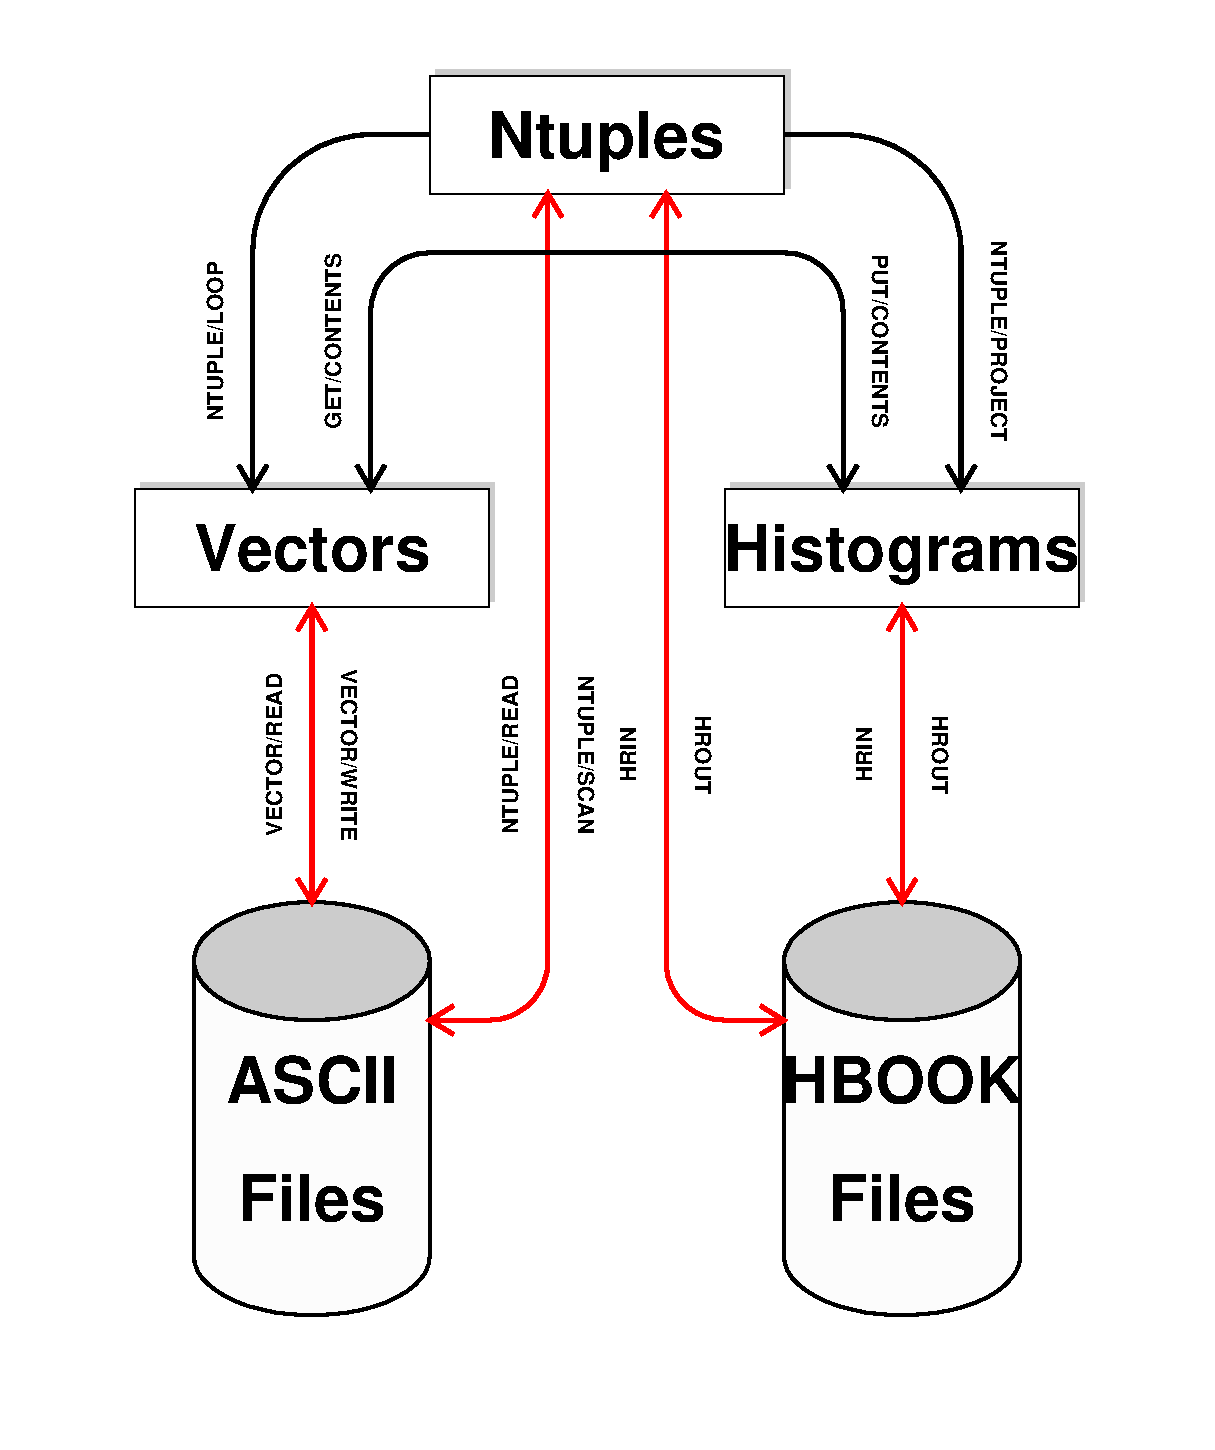
\includegraphics[width=.7\linewidth]{pawtut10.eps}
\caption{PAW entities and their related commands}
\label{fig:PAWCOM}
\end{figure}

Relations which exist between various PAW entities as described in section 
\ref{sec:pawstructure} on page~\pageref{sec:pawstructure}
and the operations which can be performed upon them have been
schematically represented in figure \ref{fig:PAWCOM}.
All commands shown in the picture next to the lines connecting the objects
have been abbreviated in a way that
they are unambiguous and can be typed to PAW, which will then
detail the various parameters to be supplied.
 
There are three main input/output formats, namely a simple text
file (e.g. with data points or commands), a direct access ZEBRA RZ file
(used by HBOOK and HIGZ for storing histograms and pictures on a given
machine) and a ZEBRA FZ sequential file, which can be used to transfer
structured ZEBRA data between various computers.
The RZ and FZ representations can be transformed into each other
using the TOALFA and FRALFA commands.
\index{ZEBRA!TOALFA}
\index{ZEBRA!FRALFA}
\index{ZEBRA!RZ file}
\index{ZEBRA!FZ file}
\index{text!data}
 
The three main PAW objects, Ntuples, histograms and vectors, can be
{\bf printed} on an alphanumeric screen (\Ucom{PRINT}
commands) or they can be plotted on a graphics screen (\Ucom{PLOT}
commands). 
The picture can be transformed into a ZEBRA data structure
and stored in a HIGZ database for later reference (e.g. editing by the
HIGZ editor), or an external presentation can be obtained via the
\index{metafile}
creation of a {\bf metafile}. 
\index{PAW!object}
\index{PRINT!commands}
\index{PLOT!commands}
\index{HIGZ}
\index{metafile}
\index{PostScript}
\index{PAW!entities}

\endinput
